\documentclass[12pt, twoside]{article}
\usepackage[letterpaper, margin=1in, headsep=0.5in]{geometry}
\usepackage[english]{babel}
\usepackage[utf8]{inputenc}
\usepackage{amsmath}
\usepackage{amsfonts}
\usepackage{amssymb}
\usepackage{tikz}
\usepackage{yhmath}
\usetikzlibrary{quotes, angles}

\usepackage{graphicx}
\usepackage{enumitem}
\usepackage{multicol}

\usepackage{fancyhdr}
\pagestyle{fancy}
\fancyhf{}
\renewcommand{\headrulewidth}{0pt} % disable the underline of the header

\fancyhead[RE]{\thepage}
\fancyhead[RO]{\thepage \\ Name: \hspace{3cm}}
\fancyhead[L]{BECA / Dr. Huson / 10th Grade Geometry\\* 7 May 2019}

\begin{document}
\subsubsection*{10.9 Do Now: Volume, density, trig review}
 \begin{enumerate}

   \item $\triangle ABC$ is shown with $m\angle C=90^\circ$ and the lengths of the triangle's sides are $BC=8$, $AC=15$, and $AB=17$.
      \begin{center}
         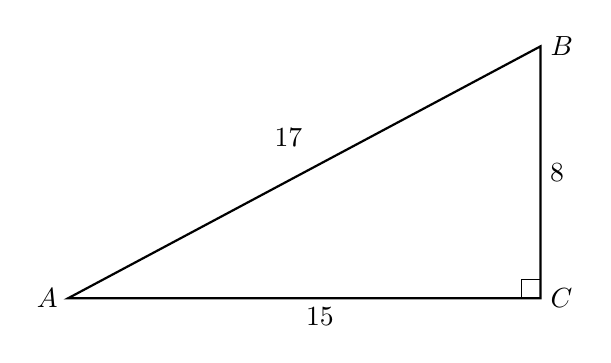
\begin{tikzpicture}[scale=0.4]
           \draw [thick]
           (0,0)node[left]{$A$}--
           (15,0)node[ right]{$C$}--
           (15,8)node[right]{$B$}--cycle;
           \draw (15,0)++(-0.6,0)--++(0,0.6)--+(0.6,0);
           \node at (8,0)[below]{$15$};
           \node at (15,4)[right]{$8$};
           \node at (7,4.5)[above]{$17$};
         \end{tikzpicture}
       \end{center}
        For each item circle True or False.
        \begin{multicols}{2}
         \begin{enumerate}
         \item \quad T \qquad F \qquad $\displaystyle \sin A = \frac{8}{15}$ \vspace{0.25cm}
         \item \quad T \qquad F \qquad $\displaystyle \cos A = \frac{15}{17}$
         \item \quad T \qquad F \qquad $\displaystyle \sin B = \frac{8}{17}$ \vspace{0.25cm}
         \item \quad T \qquad F \qquad $\displaystyle \tan B = \frac{15}{8}$
       \end{enumerate}
     \end{multicols}
  \vspace{1.25cm}

  \item Express each trigonometric ratio to the nearest thousandth and each angle measure to the nearest degree.
    \begin{multicols}{2}
      \begin{enumerate}
        \item $\tan 23^\circ =$ \vspace{0.5cm}
        \item $\cos 79^\circ =$
        \item $\sin^{-1} 0.5 =$ \vspace{0.5cm}
        \item $\cos^{-1} 0.707 =$
      \end{enumerate}
    \end{multicols} \vspace{1.25cm}

  \item In right triangle $ABC$, hypotenuse $\overline{AB}$ has a length of 26 cm, and side $\overline{BC}$ has a length of 17.6 cm. What is the measure of angle $B$, to the \emph{nearest degree}?

\newpage

   \item The triangle $DEF$ has base $DE=12$ and an area $A_{\triangle DEF}= 48$. Find the altitude of the triangle, $h$.\\[0.5cm]
   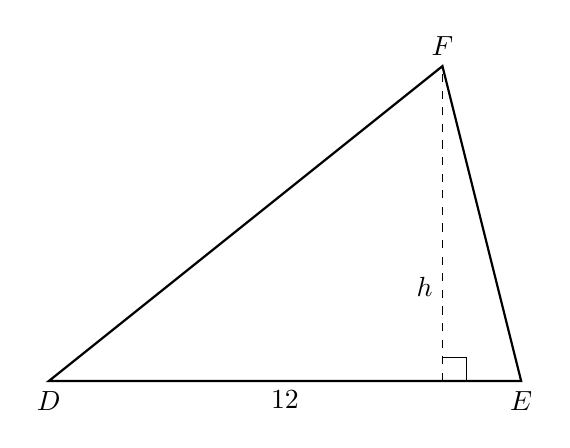
\begin{tikzpicture}[scale=1.0]
     \draw [thick]
       (0,0)node[below]{$D$}--
       (6,0)node[below]{$E$}--
       (5,4)node[above]{$F$} --cycle;
    \draw [dashed] (5,0)--(5,4);
    \draw (5,0)++(0.3,0)--++(0,0.3)--+(-0.3,0);
    \node at (5,1.2)[left]{$h$};
    \node at (3,0)[below]{$12$};
  \end{tikzpicture} \vspace{3.0cm}

  \item The base of a pyramid is a rectangle with a width of 4.6 cm and a length of 9 cm. What is the height, in centimeters, of the pyramid if its volume is 82.8 $\mathrm{cm}^3$? \vspace{4.0cm}

  \item Randy’s basketball is in the shape of a sphere with a maximum circumference of 29.5 inches. Determine and state the volume of the basketball, to the \emph{nearest cubic inch}.

  \end{enumerate}
  \newpage
  \setcounter{page}{1}
\subsubsection*{10.9 Homework: Trig review, compound volumes \& angle of elevation}
 \begin{enumerate}

  \item How many cubic inches are in the volume of a cube one foot on each side?

  \item A child’s tent can be modeled as a pyramid with a square base whose sides measure 60 inches and whose height measures 84 inches. What is the volume of the tent, to the \emph{nearest cubic foot}?

  \item Find the volume of a cylinder with radius $r=3$ and height $h=10$. Leave your answer in terms of $\pi$ (not a decimal). \vspace{2.5cm}

  \item Find the weight of $60$ liters of gasoline, given that the density of gasoline is $0.73$ kilograms per liter. \vspace{3.0cm}

  \item A circle with a diameter of 10 cm and a central angle of $30^\circ$ is drawn below.
       \begin{center}
       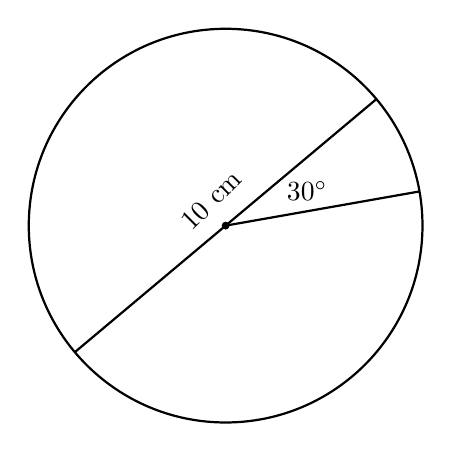
\begin{tikzpicture}[scale=.5]
         \draw [thick] (0,0) circle[radius=5];
         \draw [thick] (40:5)--(220:5);
         \draw [thick] (0,0)--(10:5);
         \fill (0,0) circle[radius=0.1];
         \draw (23:2.25) node{$30^\circ$};
         \draw (120:0.75) node[rotate=45]{$10$ cm};
         %\draw (75:1.8) node[above] {$C$};
         %\draw (290:5) node[below] {$D$};
       \end{tikzpicture}
     \end{center}
  What is the area, to the \emph{nearest tenth of a square centimeter}, of the sector formed by the $30^\circ$ angle?

\newpage
    \item A homeowner is building three steps leading to a deck, as modeled by the diagram below. All three step rises, $\overline{HA}$,  $\overline{FG}$, and  $\overline{DE}$, are congruent, and all three step runs, $\overline{HG}$,  $\overline{FE}$, and  $\overline{DC}$, are congruent. Each step rise is perpendicular to the step run it joins. The measure of $\angle CAB = 36^\circ$ and $\angle CBA = 90^\circ$.\\[0.5cm]
      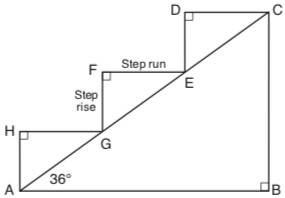
\includegraphics[width=0.4\textwidth]{steps_Aug2018-33.png}\\
    If each step run is parallel to $\overline{AB}$ and has a length of 10 inches, determine and state the length of each step rise, to the \emph{nearest tenth of an inch}.\\[3cm]
    Determine and state the length of $\overline{AC}$, to the \emph{nearest inch}.

\end{enumerate}
\end{document}

\item Theresa has a rectangular pool 30 ft long, 15 ft wide, and 4 ft deep. Theresa fills her pool using city water at a rate of \$3.95 per 100 gallons of water.\\
Nancy has a circular pool with a diameter of 24 ft and a depth of 4 ft. Nancy fills her pool with a water delivery service at a rate of \$200 per 6000 gallons.\\
If Theresa and Nancy both fill their pools 6 inches from the top of the pool, determine and state who paid more to fill her pool. ($1 \mathrm{ft}^3$ water $= 1.48$ gallons)

\item As modeled in the diagram below, an access ramp starts on flat ground and ends at the beginning of the top step. Each step is 6 inches tall and 8 inches deep. \\[0.3cm]
  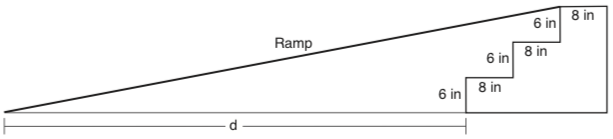
\includegraphics[width=0.8\textwidth]{ramp_Jan2019-34.png}\\
If the angle of elevation of the ramp is $4.76^\circ$, determine and state the length of the ramp, to the \emph{nearest tenth of a foot}.\\[2cm]
Determine and state, to the \emph{nearest tenth of a foot}, the horizontal distance, $d$, from the bottom of the stairs to the bottom of the ramp.
